\title{
	CSCI547 Machine Learning\\
	Homework 2\\
}
\author{
	Zachary Falkner\\
	Department of Computer Science\\
	University of Montana\\
}
\date{\today}
\documentclass[12pt]{article}

\usepackage{enumitem, listings, graphicx, xcolor, amsmath}

\lstset{language=Python,
	keywordstyle=\color{blue},
	basicstyle=\scriptsize\ttfamily,
	commentstyle=\ttfamily\itshape\color{gray},
	stringstyle=\ttfamily,
	showstringspaces=false,
	breaklines=true,
	frameround=ffff,
	frame=single,
	rulecolor=\color{black}
}

\begin{document}
	\maketitle
	
	\begin{flushleft}
		\section{Support Vector Machine}
		
		\subsection*{1A}
		
			\begin{lstlisting}
import numpy as np 
import pandas as pd

from sklearn.model_selection import train_test_split
from sklearn import svm

if __name__ == '__main__':
	DATAFILE = 'wine.data'
	
	df = pd.read_csv(DATAFILE,header=None)
	X = df.iloc[:, 1:]
	y = df.iloc[:, 0]
	
	X,X_test,y,y_test = train_test_split(X,y,test_size=0.33)
	
	clf = svm.LinearSVC()
	
	clf.fit(X, y)
	
	train_accuracy = clf.score(X, y)
	test_accuracy = clf.score(X_test, y_test)
	
	print("training accuracy: {}".format(train_accuracy))
	print("test accuracy: {}".format(test_accuracy))
			\end{lstlisting}
				
				training accuracy: 0.8571428571428571\\
				test accuracy: 0.847457627118644\\
		
		\subsection*{1B}
		
			\begin{lstlisting}
import numpy as np 
import pandas as pd

from sklearn.model_selection import train_test_split
from sklearn import svm

import matplotlib.pyplot as plt

if __name__ == '__main__':
	DATAFILE = 'wine.data'
	
	df = pd.read_csv(DATAFILE,header=None)
	X_df = df.iloc[:, 1:]
	y_df = df.iloc[:, 0]
	
	train_accuracies = []
	test_accuracies = []
	
	for i in range(100):
		X,X_test,y,y_test = train_test_split(X_df,y_df,test_size=0.33)
		
		clf = svm.LinearSVC()
		
		clf.fit(X, y)
		
		train_accuracy = clf.score(X, y)
		test_accuracy = clf.score(X_test, y_test)
		
		train_accuracies.append(train_accuracy)
		test_accuracies.append(test_accuracy)
	
	plt.hist(test_accuracies)
	plt.xlabel('Test Acuracy')
	plt.ylabel('N')
	plt.title('Distribution of Test Accuracy over 100 train/test splits')
	plt.show()

			\end{lstlisting}
			
			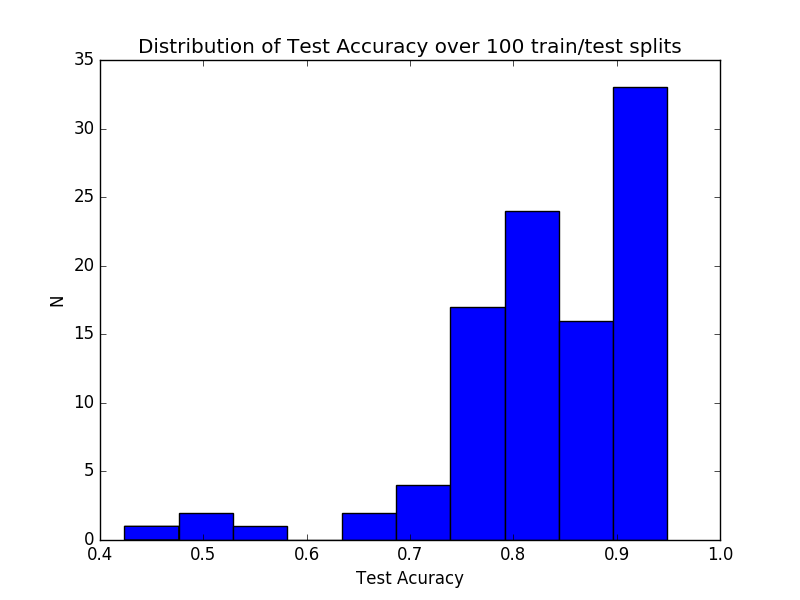
\includegraphics[scale=0.5]{HW3_1B.png}
			\label{fig:graph 1B}
		
		
		\subsection*{1C}
		
			\begin{lstlisting}
import numpy as np 
import pandas as pd

from sklearn.model_selection import train_test_split
from sklearn import svm

import matplotlib.pyplot as plt

if __name__ == '__main__':
	DATAFILE = 'wine.data'
	
	df = pd.read_csv(DATAFILE,header=None)
	X_df = df.iloc[:, 1:]
	y_df = df.iloc[:, 0]
	
	poly_test_accuracies = []
	radial_test_accuracies = []
	
	for i in range(100):
		X,X_test,y,y_test = train_test_split(X_df,y_df,test_size=0.33)
		
		clf_poly = svm.SVC(kernel='poly')
		clf_radial = svm.SVC(kernel='rbf')
		
		clf_poly.fit(X, y)
		clf_radial.fit(X, y)
		
		poly_test_accuracy = clf_poly.score(X_test, y_test)
		radial_test_accuracy = clf_radial.score(X_test, y_test)
		
		poly_test_accuracies.append(poly_test_accuracy)
		radial_test_accuracies.append(radial_test_accuracy)

	plt.hist(poly_test_accuracies)
	plt.xlabel('Test Acuracy')
	plt.ylabel('N')
	plt.title('Polynomial Test Accuracy over 100 train/test splits')
	plt.show()
	
	plt.hist(radial_test_accuracies)
	plt.xlabel('Test Acuracy')
	plt.ylabel('N')
	plt.title('Radial Test Accuracy over 100 train/test splits')
	plt.show()

			\end{lstlisting}
			
			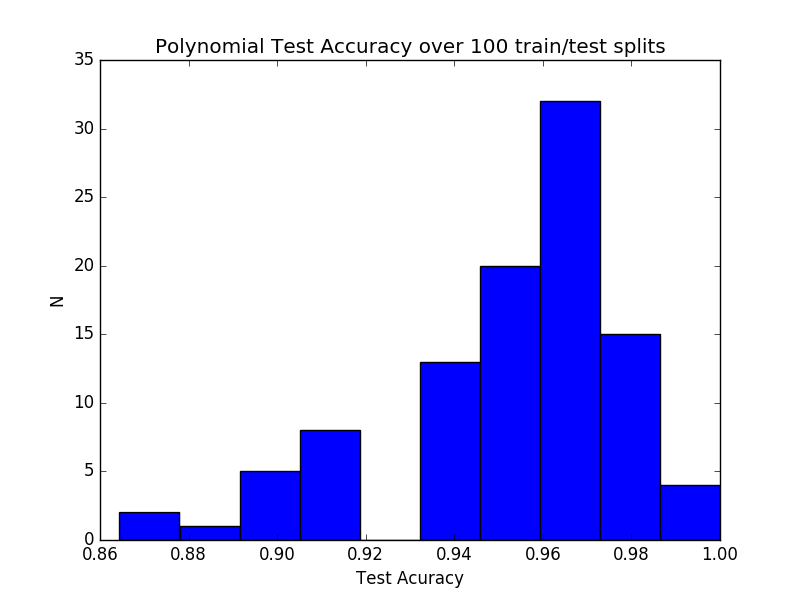
\includegraphics[scale=0.5]{HW3_1C_0.png}
			\label{fig:graph 1C.1}
			
			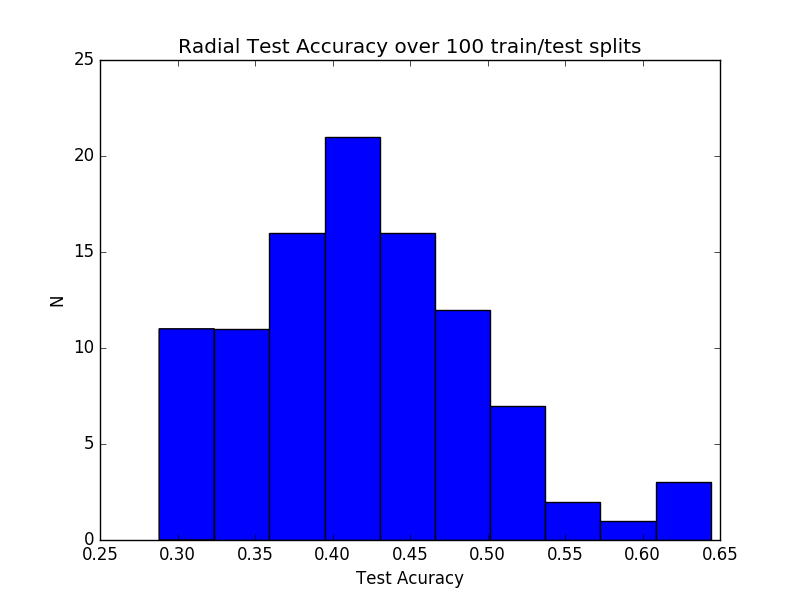
\includegraphics[scale=0.5]{HW3_1C_1.png}
			\label{fig:graph 1C.2}
			
			The polynomial kernel seems to clearly be the most robust for this dataset.\\
		
		\subsection*{1D}
		
			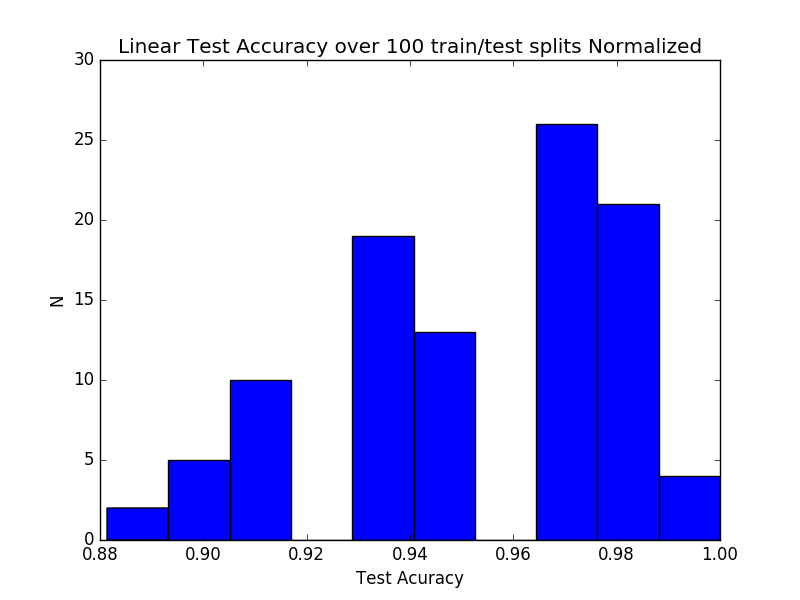
\includegraphics[scale=0.5]{HW3_1D_0.png}
			\label{fig:graph 1D.1}
			
			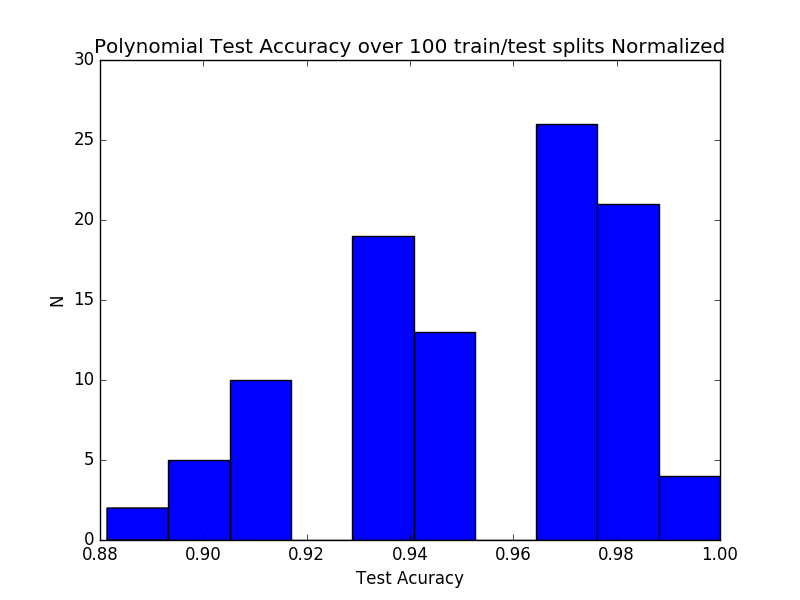
\includegraphics[scale=0.5]{HW3_1D_1.png}
			\label{fig:graph 1D.2}
			
			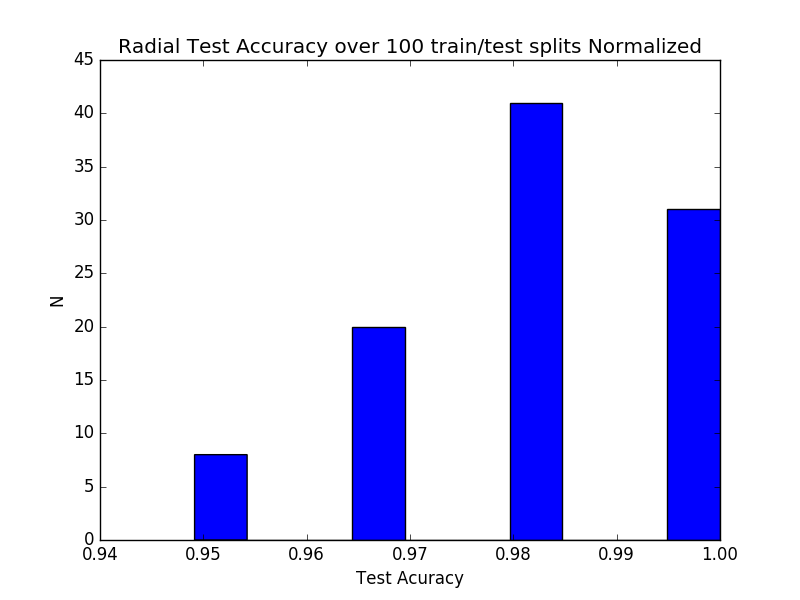
\includegraphics[scale=0.5]{HW3_1D_2.png}
			\label{fig:graph 1D.3}
			
			
			The normalization makes the performance of the radial basis go from poor to better than the polynomial or linear which had performed rather well without normalization.\\
		
		\section{Principal Component Analysis 1}
		
		\subsection*{2A}
		
			\begin{lstlisting}
import numpy as np 
import pandas as pd

import matplotlib.pyplot as plt
from mpl_toolkits.mplot3d import Axes3D

if __name__ == '__main__':
	DATAFILE1 = 'pca1.npy'
	DATAFILE2 = 'pca2.npy'
	
	data1 = np.load(DATAFILE1)
	data2 = np.load(DATAFILE2)
	
	fig = plt.figure()
	ax1 = fig.add_subplot(111, projection='3d')
	x,y,z = data1.T
	ax1.scatter(x,y,z)
	plt.show()
	
	fig = plt.figure()
	ax2 = fig.add_subplot(111, projection='3d')
	x,y,z = data2.T
	ax2.scatter(x,y,z)
	plt.show()
			\end{lstlisting}
		
			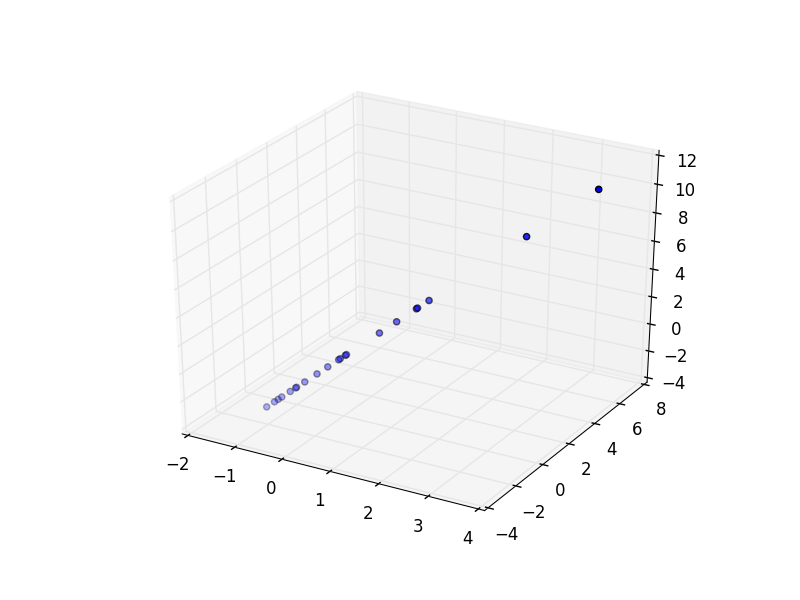
\includegraphics[scale=0.5]{HW3_2A_0.png}
			\label{fig:graph 2A.1}
			
			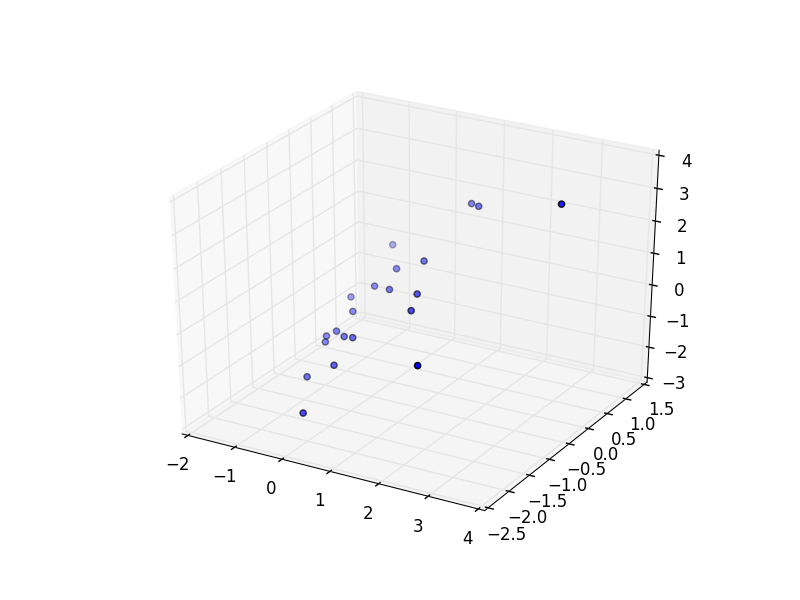
\includegraphics[scale=0.5]{HW3_2A_1.png}
			\label{fig:graph 2A.2}
			
			For the first dataset, it is pretty clear that all of the variance lies over a single axis. It is less clear with the second dataset but panning around, it appears that the variance can be explained with 2 of the 3 features.\\
		
		\subsection*{2B}
		
			\begin{lstlisting}
import numpy as np 
import pandas as pd

from sklearn.decomposition import PCA

if __name__ == '__main__':
	DATAFILE1 = 'pca1.npy'
	DATAFILE2 = 'pca2.npy'
	
	data1 = np.load(DATAFILE1)
	data2 = np.load(DATAFILE2)
	
	pca1 = PCA()
	pca1.fit(data1)
	
	pca2 = PCA()
	pca2.fit(data2)
	
	print("for {}:".format(DATAFILE1))
	print (np.cumsum(pca1.explained_variance_ratio_))
	
	print("for {}:".format(DATAFILE2))
	print (np.cumsum(pca2.explained_variance_ratio_))
			\end{lstlisting}
			
			for pca1.npy:\\
			{[ 1.  1.  1.]}\\
			for pca2.npy:\\
			{[ 0.73936844  1.          1.        ]}\\
			
			For the first dataset, all of the variance is explained by the first feature.\\
			For the second dataset, all of the variance is explained by the first 2 features.\\
			
		
		\section{Principal Component Analysis 2}
		
		\subsection*{3A}
		
			\begin{lstlisting}
from sklearn import datasets

if __name__ == "__main__":
	datasets.fetch_lfw_people(min_faces_per_person=50,resize=0.5)
	
	print("Done!")

			\end{lstlisting}
		
		\subsection*{3B}
		
			\begin{lstlisting}
import numpy as np 
import pandas as pd

from sklearn.decomposition import PCA
from sklearn import datasets
import matplotlib.pyplot as plt

if __name__ == '__main__':
	lfw_people = datasets.fetch_lfw_people(min_faces_per_person=50, resize=0.5)
	
	X = lfw_people.data
	y = lfw_people.target
	
	pca = PCA(n_components=100,copy=True,whiten=False)
	pca.fit(X)
	X = pca.transform(X)
	
	print (np.cumsum(pca.explained_variance_ratio_))
	
	fig,axs = plt.subplots(nrows=2,ncols=5)
	counter = 0
	for r in axs:
		for ax in r:
			ax.imshow(pca.components_[counter,:].reshape((62,47)))
			counter+=1
	plt.show()
			\end{lstlisting}
			
			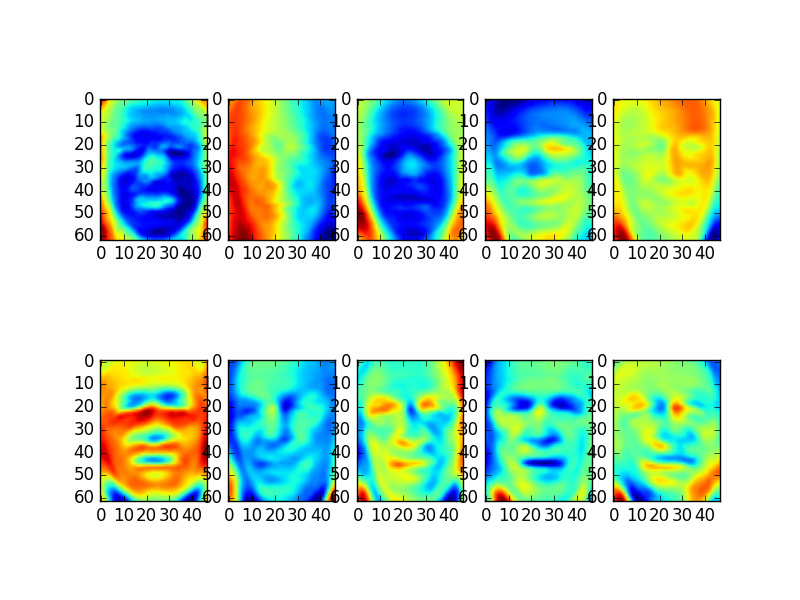
\includegraphics[scale=0.5]{HW3_3B.png}
			\label{fig:graph 3B}
		
		\subsection*{3C}
		
			\begin{lstlisting}
import numpy as np 
import pandas as pd

from sklearn.decomposition import PCA
from sklearn import datasets
import matplotlib.pyplot as plt

if __name__ == '__main__':
	lfw_people = datasets.fetch_lfw_people(min_faces_per_person=50, resize=0.5)
	
	X = lfw_people.data
	y = lfw_people.target
	
	pca1 = PCA(n_components=1,copy=True,whiten=False)
	X1 = pca1.fit_transform(X)
	
	pca10 = PCA(n_components=10,copy=True,whiten=False)
	X10 = pca10.fit_transform(X)
	
	pca100 = PCA(n_components=100,copy=True,whiten=False)
	X100 = pca100.fit_transform(X)
	
	X1_reconstructed = 0
	for c,l in zip(pca1.components_,X1[42]):
	X1_reconstructed += c*l
	X1_reconstructed += pca1.mean_
	X1_reconstructed = X1_reconstructed.reshape((62,47))
	
	X10_reconstructed = 0
	for c,l in zip(pca1.components_,X10[42]):
	X10_reconstructed += c*l
	X10_reconstructed += pca10.mean_
	X10_reconstructed = X10_reconstructed.reshape((62,47))
	
	X100_reconstructed = 0
	for c,l in zip(pca1.components_,X100[42]):
	X100_reconstructed += c*l
	X100_reconstructed += pca100.mean_
	X100_reconstructed = X100_reconstructed.reshape((62,47))
	
	fig,axs = plt.subplots(nrows=1,ncols=3)
	axs[0].imshow(X1_reconstructed)
	axs[1].imshow(X10_reconstructed)
	axs[2].imshow(X100_reconstructed)
	plt.show()

			\end{lstlisting}
			
			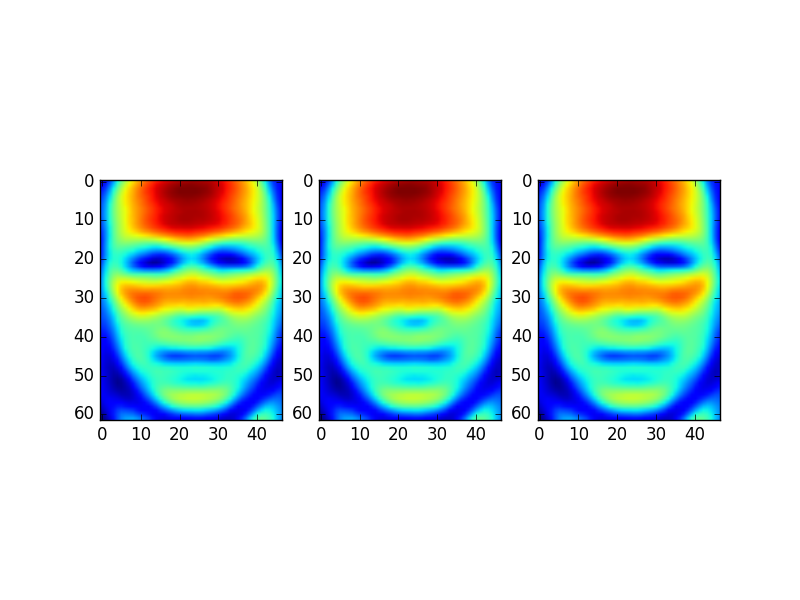
\includegraphics[scale=0.5]{HW3_3C.png}
			\label{fig:graph 3C}
			
			I feel like I should be seeing some convergence here but am not and am not sure why.\\
		
		\subsection*{3D*}
		
			\begin{lstlisting}
import numpy as np 
import pandas as pd

from sklearn.decomposition import PCA
from sklearn import datasets
import matplotlib.pyplot as plt

from sklearn.model_selection import train_test_split
from sklearn import svm
from sklearn.metrics import confusion_matrix

if __name__ == '__main__':
	lfw_people = datasets.fetch_lfw_people(min_faces_per_person=50, resize=0.5)
	
	X = lfw_people.data
	y = lfw_people.target
	
	pca = PCA(n_components=100,copy=True,whiten=True)
	X = pca.fit_transform(X)
	
	print (np.cumsum(pca.explained_variance_ratio_))
	
	X,X_test,y,y_test = train_test_split(X,y,test_size=0.33)
	
	clf = svm.LinearSVC()
	
	y_pred = clf.fit(X, y).predict(X_test)
	
	train_accuracy = clf.score(X, y)
	test_accuracy = clf.score(X_test, y_test)
	
	print("training accuracy: {}".format(train_accuracy))
	print("test accuracy: {}".format(test_accuracy))
	
	cnf_matrix = confusion_matrix(y_test, y_pred)
	print(cnf_matrix)

			\end{lstlisting}
		
			training accuracy: 0.9559808612440192\\
			test accuracy: 0.7339805825242719\\

\setcounter{MaxMatrixCols}{12}
\[
\begin{bmatrix}
14  &2   &1   &4   &1   &0   &2   &1   &2   &0   &0   &0\\
1   &59  &0   &3   &1   &2   &1   &1   &2   &0   &0   &0\\
2   &2   &23  &7   &4   &0   &0   &0   &2   &0   &1   &0\\
4   &5   &5   &146 &4   &2   &1   &0   &2   &0   &3   &4\\
0   &3   &1   &2   &22  &1   &0   &1   &2   &0   &0   &1\\
0   &1   &0   &1   &2   &18  &0   &0   &0   &1   &2   &1\\
1   &1   &0   &3   &2   &0   &2   &0   &0   &0   &1   &1\\
0   &0   &2   &1   &0   &0   &1   &9   &0   &0   &0   &0\\
1   &0   &0   &2   &2   &0   &0   &1   &12  &1   &0   &4\\
0   &1   &0   &0   &0   &0   &0   &0   &0   &22  &0   &0\\
1   &2   &0   &0   &0   &0   &1   &0   &0   &1   &11  &0\\
0   &2   &2   &3   &6   &0   &1   &1   &0   &1   &0   &40\\
\end{bmatrix}
\]
		
		
		\section{K-mean/Gaussian Mixture Models/Expectation Maximization}
		
		\subsection*{4A}
		
			\begin{lstlisting}
import numpy as np 
import pandas as pd

import matplotlib.pyplot as plt
import matplotlib.image as mpimg
from sklearn.cluster import KMeans

if __name__ == '__main__':
	IMAGEFILE = 'lenna.jpg'
	img=mpimg.imread(IMAGEFILE)
	lenna = np.array(img, dtype=np.float64) / 255
	
	w, h, d = original_shape = tuple(lenna.shape)
	assert d == 3
	image_array = np.reshape(lenna, (w * h, d))
	
	kmeans = KMeans(n_clusters=8).fit(image_array)
	labels = kmeans.predict(image_array)
	
	image = np.zeros((w, h, d))
	label_idx = 0
	for i in range(w):
	for j in range(h):
	image[i][j] = image_array[labels[label_idx]]
	label_idx += 1
	
	fig,axs = plt.subplots(nrows=1,ncols=2)
	axs[0].imshow(lenna)
	axs[1].imshow(image)
	plt.show()

			\end{lstlisting}
			
			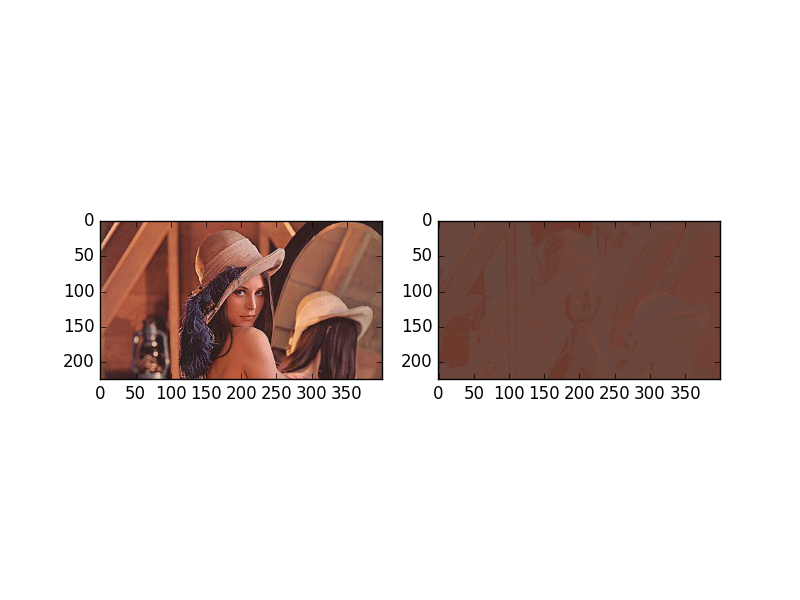
\includegraphics[scale=0.5]{HW3_4A.png}
			\label{fig:graph 4A}
		
		\subsection*{4B*}
		
			\begin{lstlisting}
...
			\end{lstlisting}
		
		
		
	\end{flushleft}
\end{document}